% Ubah judul dan label berikut sesuai dengan yang diinginkan.
\section{Metodologi}
\label{sec:metodologi}

% Ubah paragraf-paragraf pada bagian ini sesuai dengan yang diinginkan.

Tugas akhir ini merupakan penelitian yang mengintegrasikan teknologi visi komputer agar dapat mengontrol gerak kursi roda. Secara umum penelitian kali ini akan menggunakan desain sistem sesuai dengan Gambar \ref{fig:Metodologi Penelitian}.

% Gambar 3.1
\begin{figure} [ht] \centering
    % Nama dari file gambar yang diinputkan
    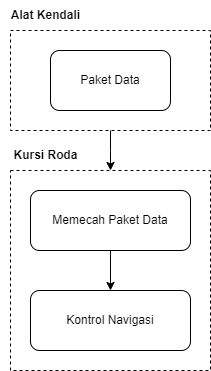
\includegraphics[scale=0.8]{gambar/DeskripsiSistem.png}
    % Keterangan gambar yang diinputkan
    \caption{Blok Diagram Penelitian}
    % Label referensi dari gambar yang diinputkan
    \label{fig:Metodologi Penelitian}
\end{figure}

\subsection{Paket Data}
Untuk dapat menggerakkan kursi roda maka perlu mengirimkan perintah ke kontroler kursi roda. Pada tahap klasifikasi pose telah didapatkan perintah dasar untuk menggerakkan kursi roda, seperti maju, mundur, kanan, kiri, maupun stop. Perintah ini kemudian akan digabungkan dengan kecepatan maksimal menjadi satu \emph{command} atau paket data seperti \("Arah, Kecepatan"\). Arah merupakan variabel dengan tipe data \emph{char} yang digunakan untuk mengatur arah gerak motor kursi roda. Kecepatan merupakan variabel dengan tipe data \emph{char} yang digunakan untuk mengatur kecepatan putar motor kursi roda.

Variabel arah memiliki tipe data \emph{char} yang akan menentukan gerak dari motor kursi roda, serta variabel kecepatan memiliki tipe data \emph{char} yang akan menentukan kecepatan maksimal dari kursi roda. Untuk memperkecil ukuran data maka kode instruksi untuk menentukan arah gerak dan kecepatan maksimal akan diwakili oleh satu huruf. Kode instruksi dapat dilihat pada Tabel \ref{tbl:kode-instruksi} dan Tabel \ref{tbl:kodePWM}. 

% Tabel 3.2
\begin{table}[h]
  \centering
      \caption{Kode Instruksi dari Hasil Klasifikasi}
      \label{tbl:kode-instruksi}
      \begin{tabular}{|c|c|}
          \hline
          Pose Classification & Instruction Code \\ \hline
          Left             & A              \\ \hline
          Forward             & B              \\ \hline
          Stop             & C              \\ \hline
          Reverse           & D              \\ \hline
          Right            & E              \\ \hline
      \end{tabular}
\end{table}


\begin{table}[!ht]
  \centering
  \caption{Kode Instruksi Untuk mengatur Tingkat PWM}
  \label{tbl:kodePWM}
  \begin{tabular}{|c|c|}
  \hline
  Maximum PWM & Instruction Code \\ \hline
  0           & O                \\ \hline
  31          & P                \\ \hline
  63          & Q                \\ \hline
  95          & R                \\ \hline
  127         & S                \\ \hline
  159         & T                \\ \hline
  191         & U                \\ \hline
  223         & V                \\ \hline
  255         & W                \\ \hline
  \end{tabular}
\end{table}

Setelah kedua variabel tersebut digabungkan maka akan dikirim secara nirkabel, baik menggunakan Bluetooth maupun WiFi dari laptop atau Jetson Nano ke ESP32.

\subsection{Memecahkan Paket Data}
Paket data yang telah dikirimkan melalui laptop maupun Jetson Nano akan diterima oleh ESP32 menggunakan Bluetooth maupun WiFi. Saat diterima oleh ESP32, data tersebut akan menjalani serangkaian proses yang melibatkan pemecahan paket data dan penyesuaian sesuai dengan variabel yang telah ditentukan sebelumnya. Pemecahan paket data ini memungkinkan ESP32 untuk mendekomposisi informasi yang terkandung dalam setiap paket dan memastikan bahwa setiap variabel terpisah dengan akurat. Dengan demikian proses ini akan mengorganisir dan menyusun kembali informasi serta memastikan bahwa setiap variabel telah benar sesuai dengan nama variabel dan tipe data yang disediakan.

\subsection{Kontrol Navigasi}
Kedua variabel yang didapatkan dari pemecahan paket data akan diproses pada ESP32. Variabel arah akan berperan untuk menentukan arah gerak dari motor, sedangkan variabel kecepatan akan digunakan untuk menetapkan kecepatan maksimal dari pergerakan motor tersebut. Terdapat serangkaian logika \emph{if} berantai pada kontrol navigasi, dimana empat variabel dir akan menentukan arah putaran motor. Selain itu, nilai PWM maksimal dikonfigurasi dengan menggunakan variabel kecepatan sehingga pengguna dapat menyesuaikan kecepatan maksimal motor yang pengguna inginkan. Dengan demikian pada tahap ini ESP32 dapat secara efektif memproses data yang diterima melalui sistem nirkabel dan menghasilkan instruksi kontrol yang sesuai untuk menggerakkan kursi roda dengan arah dan kecepatan yang diinginkan.